\documentclass[tikz]{standalone}

\usepackage{amsmath}

\usetikzlibrary{arrows,positioning}

\begin{document}
	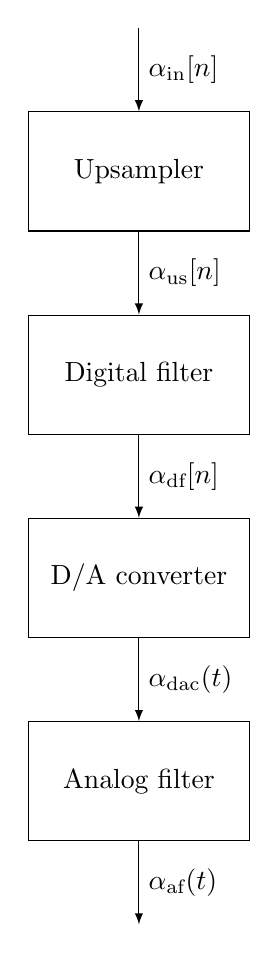
\begin{tikzpicture}[
		node distance=3em,
		arrow/.style={-latex},
		block/.style={draw, minimum height=10ex, minimum width=8em, align=center},
	]
		\coordinate (in) at (0,0);
		\node (us) [block, below=of in] {Upsampler};
		\node (df) [block, below=of us] {Digital filter};
		\node (dac) [block, below=of df] {D/A converter};
		\node (af) [block, below=of dac] {Analog filter};
		\coordinate[below=of af] (out);
		
		\draw[arrow] (in) -- node[anchor=west]{$\alpha_\text{in}[n]$} (us);
		\draw[arrow] (us) -- node[anchor=west]{$\alpha_\text{us}[n]$} (df);
		\draw[arrow] (df) -- node[anchor=west]{$\alpha_\text{df}[n]$} (dac);
			\draw[arrow] (dac) -- node[anchor=west]{$\alpha_\text{dac}(t)$} (af);
		\draw[arrow] (af) -- node[anchor=west]{$\alpha_\text{af}(t)$} (out);
	\end{tikzpicture}
\end{document}